
%%%%%%%%%%%%%%%%%% PREAMBULE %%%%%%%%%%%%%%%%%%

\documentclass[aspectratio=169,utf8]{beamer}
%\documentclass[aspectratio=169,handout]{beamer}

\usetheme{Boadilla}
%\usecolortheme{seahorse}
\usecolortheme[RGB={245,66,24}]{structure}
\useoutertheme{infolines}

% packages
\usepackage{amsfonts,amsmath,amssymb,amsthm}
\usepackage[utf8]{inputenc}
\usepackage[T1]{fontenc}
\usepackage{lmodern}

\usepackage[francais]{babel}
\usepackage{fancybox}
\usepackage{graphicx}

\usepackage{float}
\usepackage{xfrac}

%\usepackage[usenames, x11names]{xcolor}
\usepackage{tikz}
\usepackage{pgfplots}
\usepackage{datetime}



%-----  Package unités -----
\usepackage{siunitx}
\sisetup{locale = FR,detect-all,per-mode = symbol}

%\usepackage{mathptmx}
%\usepackage{fouriernc}
%\usepackage{newcent}
%\usepackage[mathcal,mathbf]{euler}

%\usepackage{palatino}
%\usepackage{newcent}
% \usepackage[mathcal,mathbf]{euler}



% \usepackage{hyperref}
% \hypersetup{colorlinks=true, linkcolor=blue, urlcolor=blue,
% pdftitle={Exo7 - Exercices de mathématiques}, pdfauthor={Exo7}}


%section
% \usepackage{sectsty}
% \allsectionsfont{\bf}
%\sectionfont{\color{Tomato3}\upshape\selectfont}
%\subsectionfont{\color{Tomato4}\upshape\selectfont}

%----- Ensembles : entiers, reels, complexes -----
\newcommand{\Nn}{\mathbb{N}} \newcommand{\N}{\mathbb{N}}
\newcommand{\Zz}{\mathbb{Z}} \newcommand{\Z}{\mathbb{Z}}
\newcommand{\Qq}{\mathbb{Q}} \newcommand{\Q}{\mathbb{Q}}
\newcommand{\Rr}{\mathbb{R}} \newcommand{\R}{\mathbb{R}}
\newcommand{\Cc}{\mathbb{C}} 
\newcommand{\Kk}{\mathbb{K}} \newcommand{\K}{\mathbb{K}}

%----- Modifications de symboles -----
\renewcommand{\epsilon}{\varepsilon}
\renewcommand{\Re}{\mathop{\text{Re}}\nolimits}
\renewcommand{\Im}{\mathop{\text{Im}}\nolimits}
%\newcommand{\llbracket}{\left[\kern-0.15em\left[}
%\newcommand{\rrbracket}{\right]\kern-0.15em\right]}

\renewcommand{\ge}{\geqslant}
\renewcommand{\geq}{\geqslant}
\renewcommand{\le}{\leqslant}
\renewcommand{\leq}{\leqslant}
\renewcommand{\epsilon}{\varepsilon}

%----- Fonctions usuelles -----
\newcommand{\ch}{\mathop{\text{ch}}\nolimits}
\newcommand{\sh}{\mathop{\text{sh}}\nolimits}
\renewcommand{\tanh}{\mathop{\text{th}}\nolimits}
\newcommand{\cotan}{\mathop{\text{cotan}}\nolimits}
\newcommand{\Arcsin}{\mathop{\text{arcsin}}\nolimits}
\newcommand{\Arccos}{\mathop{\text{arccos}}\nolimits}
\newcommand{\Arctan}{\mathop{\text{arctan}}\nolimits}
\newcommand{\Argsh}{\mathop{\text{argsh}}\nolimits}
\newcommand{\Argch}{\mathop{\text{argch}}\nolimits}
\newcommand{\Argth}{\mathop{\text{argth}}\nolimits}
\newcommand{\pgcd}{\mathop{\text{pgcd}}\nolimits} 


%----- Commandes divers ------
\newcommand{\ii}{\mathrm{i}}
\newcommand{\dd}{\text{d}}
\newcommand{\id}{\mathop{\text{id}}\nolimits}
\newcommand{\Ker}{\mathop{\text{Ker}}\nolimits}
\newcommand{\Card}{\mathop{\text{Card}}\nolimits}
\newcommand{\Vect}{\mathop{\text{Vect}}\nolimits}
\newcommand{\Mat}{\mathop{\text{Mat}}\nolimits}
\newcommand{\rg}{\mathop{\text{rg}}\nolimits}
\newcommand{\tr}{\mathop{\text{tr}}\nolimits}


%----- Structure des exercices ------

\newtheoremstyle{styleexo}% name
{2ex}% Space above
{3ex}% Space below
{}% Body font
{}% Indent amount 1
{\bfseries} % Theorem head font
{}% Punctuation after theorem head
{\newline}% Space after theorem head 2
{}% Theorem head spec (can be left empty, meaning ‘normal’)

%\theoremstyle{styleexo}
\newtheorem{exo}{Exercice}
\newtheorem{ind}{Indications}
\newtheorem{cor}{Correction}


\newcommand{\exercice}[1]{} \newcommand{\finexercice}{}
%\newcommand{\exercice}[1]{{\tiny\texttt{#1}}\vspace{-2ex}} % pour afficher le numero absolu, l'auteur...
\newcommand{\enonce}{\begin{exo}} \newcommand{\finenonce}{\end{exo}}
\newcommand{\indication}{\begin{ind}} \newcommand{\finindication}{\end{ind}}
\newcommand{\correction}{\begin{cor}} \newcommand{\fincorrection}{\end{cor}}

\newcommand{\noindication}{\stepcounter{ind}}
\newcommand{\nocorrection}{\stepcounter{cor}}

\newcommand{\fiche}[1]{} \newcommand{\finfiche}{}
\newcommand{\titre}[1]{\centerline{\large \bf #1}}
\newcommand{\addcommand}[1]{}
\newcommand{\video}[1]{}

% Marge
\newcommand{\mymargin}[1]{\marginpar{{\small #1}}}

\def\noqed{\renewcommand{\qedsymbol}{}}


%----- Presentation ------
\setlength{\parindent}{0cm}

%\newcommand{\ExoSept}{\href{http://exo7.emath.fr}{\textbf{\textsf{Exo7}}}}

\definecolor{myred}{rgb}{0.93,0.26,0}
\definecolor{myorange}{rgb}{0.97,0.58,0}
\definecolor{myyellow}{rgb}{1,0.86,0}

\newcommand{\LogoExoSept}[1]{  % input : echelle
{\usefont{U}{cmss}{bx}{n}
\begin{tikzpicture}[scale=0.1*#1,transform shape]
  \fill[color=myorange] (0,0)--(4,0)--(4,-4)--(0,-4)--cycle;
  \fill[color=myred] (0,0)--(0,3)--(-3,3)--(-3,0)--cycle;
  \fill[color=myyellow] (4,0)--(7,4)--(3,7)--(0,3)--cycle;
  \node[scale=5] at (3.5,3.5) {Exo7};
\end{tikzpicture}}
}


\newcommand{\debutmontitre}{
  \author{} \date{} 
  \thispagestyle{empty}
  \hspace*{-10ex}
  \begin{minipage}{\textwidth}
    \titlepage  
  \vspace*{-2.5cm}
  \begin{center}
    \LogoExoSept{2.5}
  \end{center}
  \end{minipage}

  \vspace*{-0cm}
  
  % Astuce pour que le background ne soit pas discrétisé lors de la conversion pdf -> png
\begin{tikzpicture}
        \fill[opacity=0,green!60!black] (0,0)--++(0,0)--++(0,0)--++(0,0)--cycle; 
\end{tikzpicture}

% toc S'affiche trop tot :
% \tableofcontents[hideallsubsections, pausesections]
}

\newcommand{\finmontitre}{
  \end{frame}
  \setcounter{framenumber}{0}
} % ne marche pas pour une raison obscure

%----- Commandes supplementaires ------

% \usepackage[landscape]{geometry}
% \geometry{top=1cm, bottom=3cm, left=2cm, right=10cm, marginparsep=1cm
% }
% \usepackage[a4paper]{geometry}
% \geometry{top=2cm, bottom=2cm, left=2cm, right=2cm, marginparsep=1cm
% }

%\usepackage{standalone}


% New command Arnaud -- november 2011
\setbeamersize{text margin left=24ex}
% si vous modifier cette valeur il faut aussi
% modifier le decalage du titre pour compenser
% (ex : ici =+10ex, titre =-5ex

\theoremstyle{definition}
%\newtheorem{proposition}{Proposition}
%\newtheorem{exemple}{Exemple}
%\newtheorem{theoreme}{Théorème}
%\newtheorem{lemme}{Lemme}
%\newtheorem{corollaire}{Corollaire}
%\newtheorem*{remarque*}{Remarque}
%\newtheorem*{miniexercice}{Mini-exercices}
%\newtheorem{definition}{Définition}

% Commande tikz
\usetikzlibrary{calc}
\usetikzlibrary{patterns,arrows}
\usetikzlibrary{matrix}
\usetikzlibrary{fadings} 

%definition d'un terme
\newcommand{\defi}[1]{{\color{myorange}\textbf{\emph{#1}}}}
\newcommand{\evidence}[1]{{\color{blue}\textbf{\emph{#1}}}}
\newcommand{\assertion}[1]{\emph{\og#1\fg}}  % pour chapitre logique
%\renewcommand{\contentsname}{Sommaire}
\renewcommand{\contentsname}{}
\setcounter{tocdepth}{2}



%------ Figures ------

\def\myscale{1} % par défaut 
\newcommand{\myfigure}[2]{  % entrée : echelle, fichier figure
\def\myscale{#1}
\begin{center}
\footnotesize
{#2}
\end{center}}


%------ Encadrement ------

\usepackage{fancybox}


\newcommand{\mybox}[1]{
\setlength{\fboxsep}{7pt}
\begin{center}
\shadowbox{#1}
\end{center}}

\newcommand{\myboxinline}[1]{
\setlength{\fboxsep}{5pt}
\raisebox{-10pt}{
\shadowbox{#1}
}
}

%--------------- Commande beamer---------------
\newcommand{\beameronly}[1]{#1} % permet de mettre des pause dans beamer pas dans poly


\setbeamertemplate{navigation symbols}{}
\setbeamertemplate{footline}  % tiré du fichier beamerouterinfolines.sty
{
  \leavevmode%
  \hbox{%
  \begin{beamercolorbox}[wd=.333333\paperwidth,ht=2.25ex,dp=1ex,center]{author in head/foot}%
    % \usebeamerfont{author in head/foot}\insertshortauthor%~~(\insertshortinstitute)
    \usebeamerfont{section in head/foot}{\bf\insertshorttitle}
  \end{beamercolorbox}%
  \begin{beamercolorbox}[wd=.333333\paperwidth,ht=2.25ex,dp=1ex,center]{title in head/foot}%
    \usebeamerfont{section in head/foot}{\bf\insertsectionhead}
  \end{beamercolorbox}%
  \begin{beamercolorbox}[wd=.333333\paperwidth,ht=2.25ex,dp=1ex,right]{date in head/foot}%
    % \usebeamerfont{date in head/foot}\insertshortdate{}\hspace*{2em}
    \insertframenumber{} / \inserttotalframenumber\hspace*{2ex} 
  \end{beamercolorbox}}%
  \vskip0pt%
}


\definecolor{mygrey}{rgb}{0.5,0.5,0.5}
\setlength{\parindent}{0cm}
%\DeclareTextFontCommand{\helvetica}{\fontfamily{phv}\selectfont}

% background beamer
\definecolor{couleurhaut}{rgb}{0.85,0.9,1}  % creme
\definecolor{couleurmilieu}{rgb}{1,1,1}  % vert pale
\definecolor{couleurbas}{rgb}{0.85,0.9,1}  % blanc
\setbeamertemplate{background canvas}[vertical shading]%
[top=couleurhaut,middle=couleurmilieu,midpoint=0.4,bottom=couleurbas] 
%[top=fondtitre!05,bottom=fondtitre!60]



\makeatletter
\setbeamertemplate{theorem begin}
{%
  \begin{\inserttheoremblockenv}
  {%
    \inserttheoremheadfont
    \inserttheoremname
    \inserttheoremnumber
    \ifx\inserttheoremaddition\@empty\else\ (\inserttheoremaddition)\fi%
    \inserttheorempunctuation
  }%
}
\setbeamertemplate{theorem end}{\end{\inserttheoremblockenv}}

\newenvironment{theoreme}[1][]{%
   \setbeamercolor{block title}{fg=structure,bg=structure!40}
   \setbeamercolor{block body}{fg=black,bg=structure!10}
   \begin{block}{{\bf Th\'eor\`eme }#1}
}{%
   \end{block}%
}


\newenvironment{proposition}[1][]{%
   \setbeamercolor{block title}{fg=structure,bg=structure!40}
   \setbeamercolor{block body}{fg=black,bg=structure!10}
   \begin{block}{{\bf Proposition }#1}
}{%
   \end{block}%
}

\newenvironment{corollaire}[1][]{%
   \setbeamercolor{block title}{fg=structure,bg=structure!40}
   \setbeamercolor{block body}{fg=black,bg=structure!10}
   \begin{block}{{\bf Corollaire }#1}
}{%
   \end{block}%
}

\newenvironment{mydefinition}[1][]{%
   \setbeamercolor{block title}{fg=structure,bg=structure!40}
   \setbeamercolor{block body}{fg=black,bg=structure!10}
   \begin{block}{{\bf Définition} #1}
}{%
   \end{block}%
}

\newenvironment{lemme}[0]{%
   \setbeamercolor{block title}{fg=structure,bg=structure!40}
   \setbeamercolor{block body}{fg=black,bg=structure!10}
   \begin{block}{\bf Lemme}
}{%
   \end{block}%
}

\newenvironment{remarque}[1][]{%
   \setbeamercolor{block title}{fg=black,bg=structure!20}
   \setbeamercolor{block body}{fg=black,bg=structure!5}
   \begin{block}{Remarque #1}
}{%
   \end{block}%
}


\newenvironment{exemple}[1][]{%
   \setbeamercolor{block title}{fg=black,bg=structure!20}
   \setbeamercolor{block body}{fg=black,bg=structure!5}
   \begin{block}{{\bf Exemple }#1}
}{%
   \end{block}%
}


\newenvironment{miniexercice}[0]{%
   \setbeamercolor{block title}{fg=structure,bg=structure!20}
   \setbeamercolor{block body}{fg=black,bg=structure!5}
   \begin{block}{Mini-exercices}
}{%
   \end{block}%
}


\newenvironment{tp}[0]{%
   \setbeamercolor{block title}{fg=structure,bg=structure!40}
   \setbeamercolor{block body}{fg=black,bg=structure!10}
   \begin{block}{\bf Travaux pratiques}
}{%
   \end{block}%
}
\newenvironment{exercicecours}[1][]{%
   \setbeamercolor{block title}{fg=structure,bg=structure!40}
   \setbeamercolor{block body}{fg=black,bg=structure!10}
   \begin{block}{{\bf Exercice }#1}
}{%
   \end{block}%
}
\newenvironment{algo}[1][]{%
   \setbeamercolor{block title}{fg=structure,bg=structure!40}
   \setbeamercolor{block body}{fg=black,bg=structure!10}
   \begin{block}{{\bf Algorithme}\hfill{\color{gray}\texttt{#1}}}
}{%
   \end{block}%
}


\setbeamertemplate{proof begin}{
   \setbeamercolor{block title}{fg=black,bg=structure!20}
   \setbeamercolor{block body}{fg=black,bg=structure!5}
   \begin{block}{{\footnotesize Démonstration}}
   \footnotesize
   \smallskip}
\setbeamertemplate{proof end}{%
   \end{block}}
\setbeamertemplate{qed symbol}{\openbox}


\makeatother
\usecolortheme[RGB={245,66,24}]{structure}

% Commande spécifique à ce chapitre

\newcommand{\Python}{\texttt{Python}}

\usepackage{textcomp}

\usepackage{listings}
\lstset{
  literate={é}{{\'e}}1
           {è}{{\`e}}1
           {à}{{\`a}}1
}


\newcommand{\codeinline}[1]{\lstinline!#1!}

%% Black and white
% \lstset{
%   upquote=true,
%   columns=flexible,
%   keepspaces=true,
%   basicstyle=\ttfamily,
%   commentstyle=\color{gray},
%   language=Python,
%   showstringspaces=false,
%   aboveskip=0em,  
%   belowskip=0em,
%   escapeinside=||
% }


%% Color
\lstset{
  language=Python,
  upquote=true,
  columns=flexible,
  keepspaces=true,
  basicstyle=\ttfamily,
  commentstyle=\color{gray},
  keywordstyle=\color{blue},
  %emph={bin,oct,hex},
  emphstyle=\color{blue},
  stringstyle=\color{Green4},
  frame=single,  
  showspaces=false,
  showstringspaces=false,
  literate={>>>}{\textcolor{red}{>\,\!>\,\!>}}{3},
}


\renewcommand{\debutmontitre}{
  \author{} \date{} 
  \thispagestyle{empty}
  \hspace*{-10ex}
  \begin{minipage}{\textwidth}
    \titlepage  
  \vspace*{-1.5cm}
%   \begin{center}
%     \LogoExoSept{2.5}
%   \end{center}
  \end{minipage}

  \vspace*{-0cm}
  
  % Astuce pour que le background ne soit pas discrétisé lors de la conversion pdf -> png
\begin{tikzpicture}
        \fill[opacity=0,green!60!black] (0,0)--++(0,0)--++(0,0)--++(0,0)--cycle; 
\end{tikzpicture}

% toc S'affiche trop tot :
% \tableofcontents[hideallsubsections, pausesections]
}

%%%%%%%%%%%%%%%%%%%%%%%%%%%%%%%%%%%%%%%%%%%%%%%%%%%%%%%%%%%%%
%%%%%%%%%%%%%%%%%%%%%%%%%%%%%%%%%%%%%%%%%%%%%%%%%%%%%%%%%%%%%


\begin{document}


\title{{\bf Représentation des nombres}}
\subtitle{Représentation des nombres entiers en base $2$}

\begin{frame}
  
  \debutmontitre

  \pause

{\footnotesize
\hfil\qquad\qquad\qquad\qquad
\setbeamercovered{transparent=50}
\begin{minipage}{0.6\textwidth}
  \begin{itemize}
    \item<3-> Objectifs du chapitre
    \item<4-> Motivation
    \item<5-> Les puissances de $2$
    \item<6-> \'Ecriture binaire 
    \item<7-> Bits et octets
    \item<8-> Mesures de quantité de mémoire   
  \end{itemize}
\end{minipage}
}

\end{frame}

\setcounter{framenumber}{0}

%%%%%%%%%%%%%%%%%%%%%%%%%%%%%%%%%%%%%%%%%%%%%%%%%%%%%%%%%%%%%%%%
\section{Objectifs du chapitre}

\begin{frame}

\evidence{Objectifs du chapitre}

\begin{itemize}
\item<2-> Savoir ce que sont les représentations de nombres entiers en base $2$, $8$  et $16$
\item<3-> Savoir convertir un nombre entier dans l'une de ces bases
\item<4-> Savoir calculer l'entier connaissant sa représentation dans l'une de ces bases
\item<5-> Connaître les fonctions de \Python\ permettant ces conversions
\item<6->     Savoir les programmer
\end{itemize} 
\end{frame}



%%%%%%%%%%%%%%%%%%%%%%%%%%%%%%%%%%%%%%%%%%%%%%%%%%%%%%%%%%%%%%%%
\section{Motivation}

\begin{frame}

\evidence{Motivation}

\begin{itemize}
  \item<2-> L'écriture des nombres s'effectue de plusieurs façons
  
  \item<3-> Le nombre quarante-sept peut s'écrire
  
\begin{itemize}
\item<4-> avec des petits traits :
{\bf\color{red}
\textbar{}\textbar{}\textbar{}\textbar{}\textbar{} \textbar{}\textbar{}\textbar{}\textbar{}\textbar{} \textbar{}\textbar{}\textbar{}\textbar{}\textbar{} \textbar{}\textbar{}\textbar{}\textbar{}\textbar{} \textbar{}\textbar{}\textbar{}\textbar{}\textbar{} \textbar{}\textbar{}\textbar{}\textbar{}\textbar{} \textbar{}\textbar{}\textbar{}\textbar{}\textbar{} \textbar{}\textbar{}\textbar{}\textbar{}\textbar{} \textbar{}\textbar{}\textbar{}\textbar{}\textbar{} \textbar{}\textbar{}
}
\item<5-> avec la numération romaine : {\bf\color{red}\codeinline{XLVII}} 
\item<6-> avec la numération décimale en utilisant les $10$ chiffres usuels : {\bf\color{red}\codeinline{47}}
\end{itemize}

  \item<7-> Un système d'écriture des nombres se décrit
  \begin{itemize}
    \item<8-> en précisant les symboles utilisés (l'alphabet)
    \item<9-> et les règles d'association de ces symboles
  \end{itemize}
\end{itemize}
\end{frame}


\begin{frame}


\evidence{Système de numération décimale}

\begin{itemize}
  \item<2-> L'alphabet est constitué de dix symboles :  
  
  \centerline{$0$, $1$, $2$, $3$, $4$, $5$, $6$, $7$, $8$ et $9$}
  
  \item<3-> À l'aide de ces dix symboles, on écrit n'importe quel nombre entier
  
  \item<4-> Le nombre quarante-sept s'écrit $47$ en base $10$
  
  \item<5-> Il est égal à $4\times 10^1 + 7\times 10^0$
  
  \item<6-> $3010 = 3\times 10^3 + 0\times 10^2 + 1\times 10^1 + 0\times 10^0$  
\end{itemize}

\end{frame}


\begin{frame}

\evidence{Pourquoi abandonner le décimal ?}



\begin{itemize}
  \item<2-> 1645~:  pascaline de Blaise Pascal. Nombres représentés en base $10$


\begin{center}
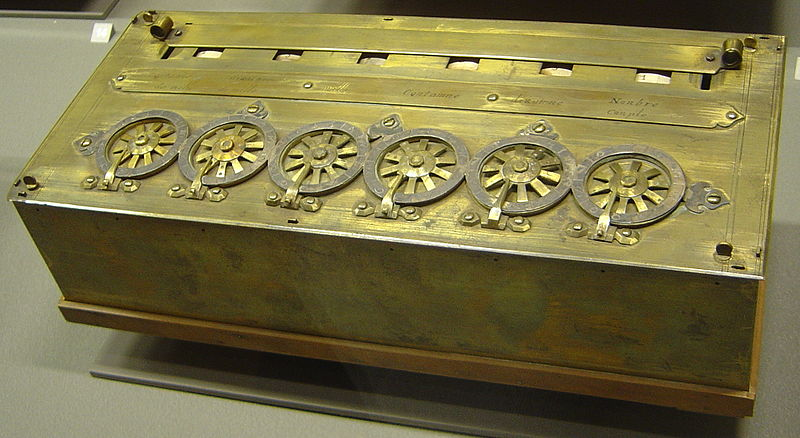
\includegraphics[scale=0.25]{Pascaline.jpg}
\end{center}  

  \item<3-> Pour les transistors : seulement deux états
  
  \item<4-> Le binaire convient mieux aux machines électroniques
\end{itemize}

\end{frame}


%%%%%%%%%%%%%%%%%%%%%%%%%%%%%%%%%%%%%%%%%%%%%%%%%%%%%%%%%%%%%%%%
\section{Les puissances de $2$}



\begin{frame}

\evidence{Puissances de $10$}

\pause
$1$, $10$, $100$, $1000$,... 

\medskip
\pause
\evidence{Puissances de $2$}
\begin{center}
\begin{tabular}{cc}
$n$&$2^n$\\\hline
0&1\\
1&2\\
2&4\\
3&8\\
4&16\\
5&32\\
6&64\\
7&128\\
8&256\\
9&512\\
10&1024\\
\end{tabular}\qquad\qquad\qquad
\begin{tabular}{cc}
$n$&$2^n$\\\hline
11&2048\\
12&4096\\
13&8192\\
14&16384\\
15&32768\\
16&65536\\
17&131072\\
18&262144\\
19&524288\\
20&1048576
\end{tabular}
\end{center}

\end{frame}



%%%%%%%%%%%%%%%%%%%%%%%%%%%%%%%%%%%%%%%%%%%%%%%%%%%%%%%%%%%%%%%%
\section{\'Ecriture binaire}




\begin{frame}

\evidence{Écriture binaire}

\pause

\mybox{
\begin{minipage}{0.8\textwidth}
\centering
Tout nombre entier admet une unique décomposition 
en somme de puissances de $2$ 
\end{minipage}
}


\begin{itemize}
  \pause
  \item $47 = 32 + 8 + 4 + 2 + 1 = 2^5 + 2^3 + 2^2 + 2^1 + 2^0$
  \pause
  \item $47
= {\color{red}1}\times 2^5 
+ {\color{red}0}\times 2^4
+ {\color{red}1}\times 2^3 
+ {\color{red}1}\times 2^2 
+ {\color{red}1}\times 2^1 
+ {\color{red}1}\times 2^0$
  \pause
  \item L'écriture en binaire est 
  $47 = \overline{{\color{red}\mathtt{101111}}}_2$
\end{itemize}


\bigskip

\begin{itemize}
  \pause
  \item $3010 = 2048 + 512 + 256 + 128 + 64 + 2$
  
    \pause
  \item $3010 = {\color{red}1}\times 2^{11}
+ {\color{red}0}\times 2^{10}
+ {\color{red}1}\times 2^9 
+ {\color{red}1}\times 2^8 
+ {\color{red}1}\times 2^7 
+ {\color{red}1}\times 2^6
+ {\color{red}0}\times 2^5
+ {\color{red}0}\times 2^4
+ {\color{red}0}\times 2^3
+ {\color{red}0}\times 2^2
+ {\color{red}1}\times 2^1
+ {\color{red}0}\times 2^0$

\pause
  \item $3010 = \overline{{\color{red}\mathtt{101111000010}}}_2$
\end{itemize}

\end{frame}



\begin{frame}

\evidence{Les nombres de $0$ à $7$}


\begin{center}
\begin{tabular}{rr}
$0$ & $\overline{\mathtt{0}}_2$ \\
$1$ & $\overline{\mathtt{1}}_2$ \\
$2$ & $\overline{\mathtt{10}}_2$ \\
$3$ & $\overline{\mathtt{11}}_2$ \\
$4$ & $\overline{\mathtt{100}}_2$ \\
$5$ & $\overline{\mathtt{101}}_2$ \\
$6$ & $\overline{\mathtt{110}}_2$ \\
$7$ & $\overline{\mathtt{111}}_2$ \\
\end{tabular}
\end{center}

\end{frame}




%%%%%%%%%%%%%%%%%%%%%%%%%%%%%%%%%%%%%%%%%%%%%%%%%%%%%%%%%%%%%%%%
\section{Bits et octets}


\begin{frame}

\evidence{Bits et octets}

\begin{itemize}
  \item<2-> Les chiffres binaires $0$ et $1$ sont appelés \defi{bits} (\emph{binary digit})
  
  \item<3-> Avec trois bits : les entiers de $0=\overline{\mathtt{000}}_2$ 
  à $7=\overline{\mathtt{111}}_2$
  
  \item<4-> Un \defi{octet} est un nombre qu'on peut écrire en binaire sur huit
bits

  \item<5-> Ce sont les entiers compris entre $0$ et $255=\overline{\mathtt{11111111}}_2$

  \item<6-> \textbf{Attention \!!} En anglais \emph{byte} désigne ce qu'en français on nomme octet
\end{itemize}

\end{frame}


%%%%%%%%%%%%%%%%%%%%%%%%%%%%%%%%%%%%%%%%%%%%%%%%%%%%%%%%%%%%%%%%
\section{Mesures de quantité de mémoire}


\begin{frame}

\begin{center}

\evidence{Puissances de $10$}

\medskip

\begin{tabular}{lll}
Nom&Puissance&Abbréviation\\
\hline
kilooctet&$10^3$&ko\\
megaoctet&$10^6$&Mo\\
gigaoctet&$10^9$&Go\\
téraoctet&$10^{12}$&To\\
pétaoctet&$10^{15}$&Po
\end{tabular}

\bigskip
\pause

\evidence{Puissances de $2$}

\medskip

\begin{tabular}{lll}
Nom&Puissance&Abbréviation\\
\hline
kibioctet&$2^{10}$&Kio\\
mébioctet&$2^{20}$&Mio\\
gibioctet&$2^{30}$&Gio\\
tébioctet&$2^{40}$&Tio\\
pébioctet&$2^{50}$&Pio
\end{tabular}
\end{center}

\end{frame}




\end{document}
